\PassOptionsToPackage{unicode}{hyperref}
\documentclass[aspectratio=1610, professionalfonts, 9pt]{beamer}

\usefonttheme[onlymath]{serif}
\usetheme[showtotalframes]{tudo}

\usepackage{hyperref}

\ifluatex
  \usepackage{polyglossia}
  \setmainlanguage{german}
\else
  \ifxetex
    \usepackage{polyglossia}
    \setmainlanguage{german}
  \else
    \usepackage[german]{babel}
  \fi
\fi

\newcommand*\xRightarrow[2][]{\ext@arrow 0359\Rightarrowfill@{#1}{#2}}

% Mathematik
\usepackage{amsmath}
\usepackage{amssymb}
\usepackage{mathtools}
\usepackage{cancel}

\usepackage{hyperref}
\usepackage{bookmark}
\usepackage{siunitx}
\usepackage{overpic}
%%%%%%%%%%%%%%%%%%%%%%%%%%%%%%%%%%%%%%%%%%%%%%%%%%%%%%%%%%%%%%%%%%%%%%%%%%%%%%%%
%%%%%-------------Hier Titel/Autor/Grafik/Lehrstuhl eintragen--------------%%%%%
%%%%%%%%%%%%%%%%%%%%%%%%%%%%%%%%%%%%%%%%%%%%%%%%%%%%%%%%%%%%%%%%%%%%%%%%%%%%%%%%

%Titel:
\title{Stromnetz und Strombörse}
%Autor
\author[D.~Hering]{Dag-Björn Hering}
%Lehrstuhl/Fakultät
%\institute[Experimental Physics 5]{Names des Lehrstuhls \\  Name der Fakultät}
%Titelgrafik
\titlegraphic{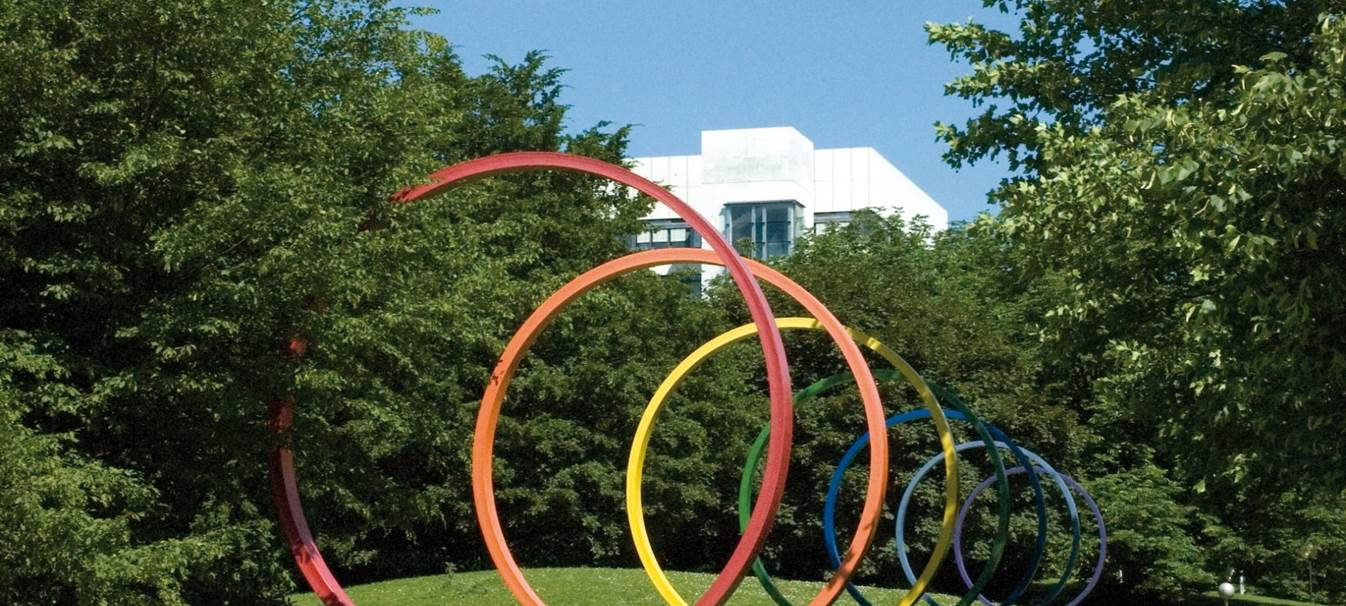
\includegraphics[width=0.7\textwidth]{images/tudo-title-2.jpg}}


\begin{document}
\maketitle

\begin{frame}{Gliederung}
\begin{itemize}
  \item[] \textbf{\textcolor{tugreen}{Stromnetz}}
  \begin{itemize}
  \item Historie
  \item Verbundnetze
  \item Spannungsebenen
  \item Netzfrequenz
  \item Stromnetz und Energiewende
  \end{itemize}
  \item[] \textbf{\textcolor{tugreen}{Strombörse}}
  \begin{itemize}
    \item Angebote der Strombörse
    \item Strompreis
    \item Erneuerbare-Energie-Gesetz
    \item Strompreisentwicklung
  \end{itemize}
\end{itemize}
\end{frame}





\begin{frame}{Stromnetz-Historisch}
\begin{itemize}
  \item Beginn der Elektrifizierung 1880 mit der Industrialisierung
  \item zunächst nur Inselnetze mit Gleichstrom zur Beleuchtung
  \item Wechselstrom setzte sich gegen Gleichstrom durch
  \item Ursachen:
  \begin{itemize}
    \item[-] damals war der Transformator die einzige Möglichkeit, Hochspannung zu erzeugen
    \item[$\rightarrow$] einfaches Umspannen von Hochspannung zu Verbraucherspannung möglich,
    somit weniger Verluste bei langen Leitungen und "sichere" Niederspannung bei Verbraucher
    \item[-] große Verbundnetze möglich, die aber alle synchron mit gleicher Frequenz betrieben werden
  \end{itemize}
  \item heutige Verbundnetze werden mit $\SI{50}{\hertz}$ bzw. $\SI{60}{\hertz}$ Drehstrom(Dreiphasiger Wechselstrom) betrieben
  % \item Nur vereinzelt Gleichstrom (z. B. bei Verkehr und HGÜ) jedoch wieder steigend
\end{itemize}
\end{frame}
%

\begin{frame}{Dreiphasiger Wechselstrom}
  \begin{columns}
    \begin{column}{0.5\textwidth}
\begin{itemize}
  \item drei Wechselströme, die um $\SI{120}{\degree}$ zueinander verschoben sind
  \item einfache Erzeugung durch Drehstromgenerator
  \item Steckdosen zu Hause benutzten jeweils nur eine der drei Wechselströme
  \item bzw. Öfen und Motoren nutzen alle drei Phasen (konstante Leistung)
  \item Materialaufwand für Leitung geringer als bei einphasigem Wechselstrom bei gleicher Leistung,
   da Phasen in separaten Kabeln geführt werden
  \item besitzt zwei abgreifbare Spannungen  Nennspannung (Phase-Phase) und Phasenspannung (Phase-Null)
\end{itemize}
\end{column}
\begin{column}{0.5\textwidth}
\centering
\includegraphics[width=0.9\textwidth]{images/Drehstromgenerator.jpg} \ \textbf{\textcolor{tugreen}{[1]}}
%www.c-turbines.ch
\end{column}
\end{columns}
\end{frame}

{
\setbeamertemplate{footline}{}
\begin{frame}{Die Europäischen Verbundsysteme}
\begin{columns}
\begin{column}{0.5\textwidth}
\begin{itemize}
\item besteht aus mehreren voneinander getrennten Verbundsystemen
\item Verbundsystem:
Zusammenschluss von Höchst- und Hochspannungsnetzen der Länder  z. B. UCTE  (Union for the Co-ordination of the Transmission of Electricity)
%\item Verbundnetze werden mit Drehstrom betrieben (Drehstrom $\stackrel{^}{=}$ 3-phasigen Wechselstrom)
\item Verband Europäischer Übertragungsnetzbetreiber
European Network of Transmission System (ENTSO-E) übernimmt Koordination
der Verbundsysteme
\end{itemize}
\end{column}
\begin{column}{0.5\textwidth}
\centering
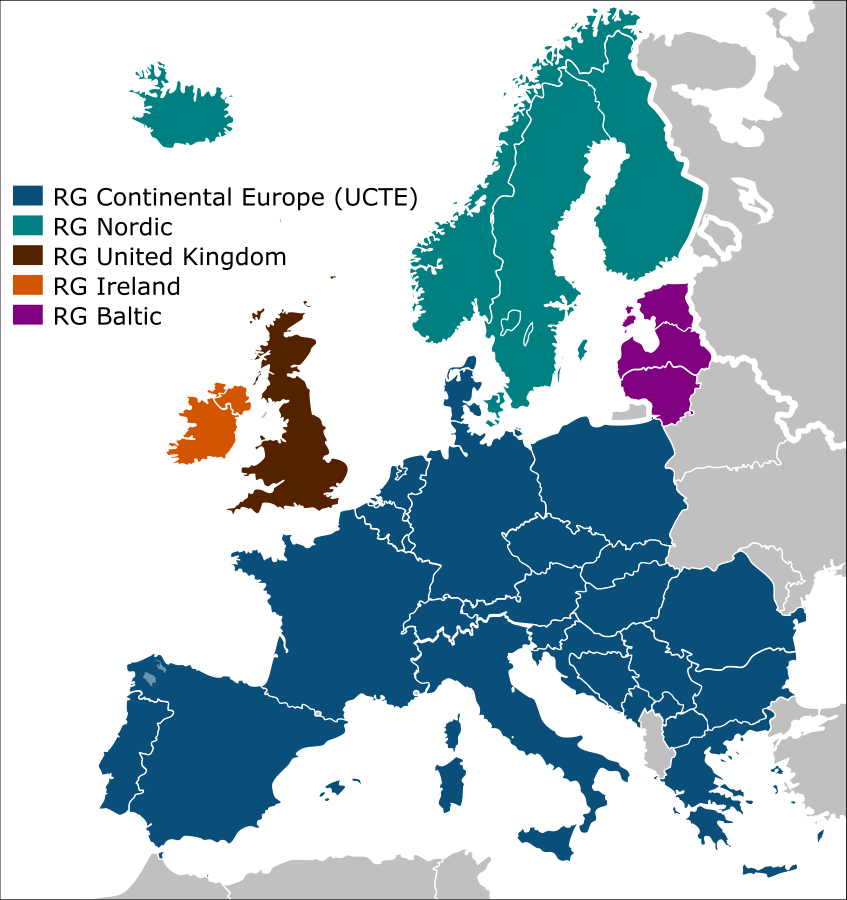
\includegraphics[width=0.9\textwidth]{images/Euronetz.png} \ \textbf{\textcolor{tugreen}{[2]}}
\end{column}
\end{columns}
% Quelle: https://commons.wikimedia.org/w/index.php?curid=1387849
\end{frame}
}


  \begin{frame}

  \begin{block}{Hochspannungs-Gleichstrom-Übertragung (HGÜ)}
    \begin{itemize}
      \item dient zur Energieübertragung zwischen zwei weit entfernten Punkten
      \item ab $\SI{600}{\kilo\meter}$ wirtschaftlicher als Freileitungen mit Wechselstrom (Bei Erdleitung bereits bei $\SI{80}{\kilo\meter}$) \footnote{\url{https://www.siemens.com/press/pool/de/events/2012/energy/2012-07-wismar/factsheet-hgue-d.pdf}}
  \item[] \textbf{\textcolor{tugreen}{Ursache:}} HGÜ: ohmscher Widerstand
  \item[] \textbf{\textcolor{tulight}{Ursache:}} Wechselstrom: ohmscher Widerstand, Skin-Effekt, kapazitiver Widerstand und Blindwiderstand
%Quelle:https://www.weltderphysik.de/gebiete/technik/energie/speichern-und-transportieren/strom/hochspannung/
% \begin{tabular}{c c}
%  AC    &          DC \\
% \hline
% \multicolumn{2}{c}{OhmscherWiderstand}\\
% Skin-Effekt &  - \\
% BlindWiderstand& -\\
%  \end{tabular}
% \begin{itemize}
      \item verbindet die getrennten und asynchronen Verbundsysteme Europas und bspw. Offshore-Windparks mit dem Festland
      \end{itemize}
\end{block}
\end{frame}

{
\setbeamertemplate{footline}{}
\begin{frame}
\begin{columns}
\begin{column}{0.4\textwidth}
\begin{overpic}[width=0.9\textwidth]
  {images/HGUeuropa.png}
  \put(55,5){\textbf{\textcolor{tugreen}{[3]}}}
\end{overpic}
\end{column}
\begin{column}{0.6\textwidth}
  \begin{overpic}[width=1\textwidth]
    {images/HGU.PNG}
    \put(95,2){\textbf{\textcolor{tugreen}{[4]}}}
  \end{overpic}
\end{column}
\end{columns}
\end{frame}
}


{
\setbeamertemplate{footline}{}
\begin{frame}
  \begin{columns}
\begin{column}{0.6\textwidth}
  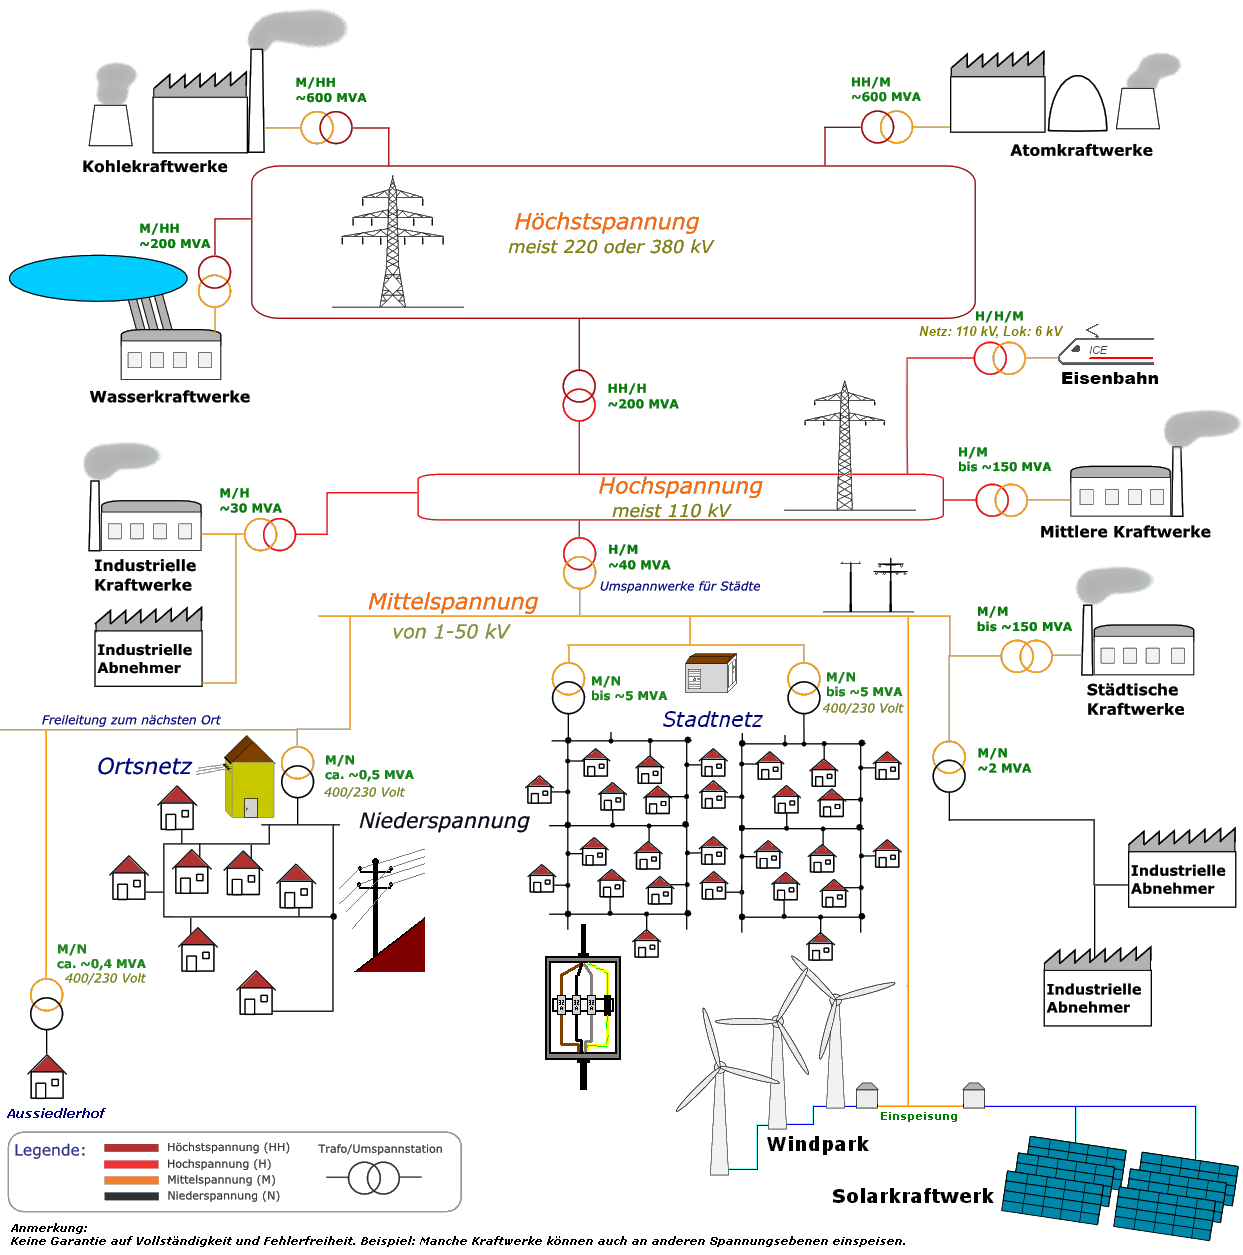
\includegraphics[width=1\textwidth]{images/Stromversorgung.png} \textbf{\textcolor{tugreen}{[5]}}
\end{column}
\begin{column}{0.4\textwidth}
  %\frametitle{Netzebenen}
  \begin{itemize}
    \item besteht aus \num{7} Netzebenen
    \item \num{4} Spannungsebenen
    \begin{itemize}
      \item[-] Höchstspannung $\num{220}$-$\SI{380}{\kilo\volt}$
      \item[-] Hochspannung  $\num{60}$-$\SI{110}{\kilo\volt}$
      \item[-] Mittelspannung  $\num{6}$-$\SI{50}{\kilo\volt}$
      \item[-] Niederspannung $\num{230}$/$\SI{400}{\volt}$
    \end{itemize}
    \item \num{3} Transformationsebenen jeweils zwischen den Spannungsebenen
    \item Höchstspannung für möglichst verlustarme Leitung
          \begin{align*}
P_{\text{Verlust}}&= U_\text{R}\cdot I = R \cdot I^2 = \rho\cdot\frac{l}{A} \cdot I^2  \\
P_\text{ges}&=U\cdot I \Leftrightarrow I=\frac{P_\text{ges}}{U}\\
P_{\text{Verlust}}&=\rho\cdot\frac{l}{A} \cdot \frac{P_\text{ges}^2}{U^2}
          \end{align*}

  \end{itemize}
\end{column}
\end{columns}
\end{frame}
}




\begin{frame}
  \begin{columns}
  \begin{column}{0.5\textwidth}
  \begin{itemize}
    \item die Höchstspannung Ebene teilen sich in
    Deutschland die Übertragungsnetzbetreiber
    \begin{itemize}
      \item[-] Tennet
      \item[-] 50-Hertz
      \item[-] Amprion
      \item[-] Transnet
    \end{itemize}
    \item Hoch-/Mittel-/Niederspannungs Ebenen
     werden regional und lokal von Verteilernetzbetreibern verwaltet
\end{itemize}
\end{column}
\begin{column}{0.5\textwidth}
\begin{overpic}[width=1\textwidth]
  {images/UNB.jpg}
\put(90,5){\textbf{\textcolor{tugreen}{[6]}}}
\end{overpic}
  %Quelle:http://www.bpb.de/politik/wirtschaft/energiepolitik/148524/ausbau-des-stromnetzes
\end{column}
\end{columns}
\end{frame}

\begin{frame}{Netzfrequenz}
\begin{itemize}% [<+->]
\item Richtfrequenz von $\SI{50}{\hertz}$ im europäischen Verbundnetz $\SI{60}{\hertz}$ im nordamerikanischen Verbundnetz
\item hängt von Rotationsgeschwindigkeit der synchronisierten Generatoren
ab
% Um dieses umgangssprachlicher zu erklären, wird
% gerne der Alltagsvergleich mit einem Fahrrad herangezogen:
% Auf einer gleichmässigen Fläche kann relativ einfach eine
% konstante Trittgeschwindigkeit gehalten werden.
% An einer Steigung (zu vergleichen mit steigender Last im Stromnetz)
% muss mehr Kraft aufgewendet werden, um die Trittfrequenz
% beizubehalten oder sie kann sogar (kurzeitig) sinken,
% bis man sich auf die Steigung eingestellt hat.
% Anders herum steigt die (Tritt-)Frequenz an einem Gefälle
% kurz an, bis man sie (zum Beispiel durch Bremsen) wieder
% auf die „normale“ Nennfrequenz gesenkt hat.
% \begin{itemize}[<+->]
%   \item test ...
%   \item test 2
% \end{itemize}
%führen
\item im Stromnetz kann keine Energie gespeichert werden
  \begin{itemize}
    \item[\rightarrow]  erzeugter Leistung $\stackrel{!}{=}$ abgenommene Leistung
  \end{itemize}
  \item Schwankungen in der Relation von abgenommener
  und erzeugter Leistung erzeugt Abweichungen in der Frequenz
  \item zu starke Abweichungen können Zerstörung der Generatoren und anderen Geräten führen
  \item Leistungsflüsse in den Netzen werden durch Änderung
    von Blind- und Wirkleistung sowie durch Phasenverschiebungen
    zur Netzstablilisierung angepasst
    (FACTS Flexible AC Transmission Systems)

\end{itemize}
\end{frame}

{
\setbeamertemplate{footline}{}
\begin{frame}
  \begin{overpic}[width=0.9\textwidth]
    {images/Frequenz.png}
\put(90,5){\textbf{\textcolor{tugreen}{[7]}}}
\end{overpic}
%Quelle:http://www.netzfrequenz.info/aktuelle-netzfrequenz-full
\end{frame}
}

\begin{frame}{Regelung der Netzfrequenz}
Notwendigkeit von regelbarer Leistung, um Frequenz konstant zu halten
\begin{itemize}
  \item positive Regelenergie:
  \begin{itemize}
    \item[-] mehr Strom muss in das Netz eingespeist werden
    \item[-] weniger Strom muss verbraucht werden
  \end{itemize}
  \item negative Regelenergie:
  \begin{itemize}
    \item[-] Stromeinspeisung muss schnell reduziert werden
    \item[-] mehr Strom muss verbraucht werden
  \end{itemize}
  \item[\rightarrow] Kraftwerke oder Verbraucher mit einer diesen Eigenschaften eignen sich, um Regelenergie bereitzustellen
\end{itemize}
\end{frame}

\begin{frame}
  \begin{itemize}
    \item Primärregelung PRL
    \begin{itemize}
      \item[-] automatische vollständige Aktivierung innerhalb von \SI{30}{\second}
      \item[-] abzudeckender Zeitraum \num{0}-\SI{15}{\minute}
      \item[-] Bereitstellung durch alle ÜNB im ENTSO-E-Gebiet
      \item[-] Frequenzabhängige Lasten vorteilhaft z. B. Asynchronmotor
      % \item[-] ?keine Unterscheidung zwischen positiver und negativer Regelenergie?
    \end{itemize}
    \item Sekundärregelung SRL
    \begin{itemize}
      \item[-] automatische Aktivierung durch betroffenen ÜNB
      \item[-] vollständige Aktivierung innerhalb von \SI{5}{\minute}
      \item[-] Unterscheidung zwischen positiver und negativer Regelenergie
      \item[-] Bereitstellung durch z. B. Pumpspeicherkraftwerken, Gasturbinen, Biogasanlagen oder Blockheizkraftwerke
    \end{itemize}
    \end{itemize}

\end{frame}


{
\setbeamertemplate{footline}{}
\begin{frame}
\begin{itemize}
\item Tertiärregelung(Minutenreserve) MRL
\begin{itemize}
  \item[-] Aktivierung innerhalb von \SI{15}{\minute}
  \item[-] abzudeckender Zeitraum mehrere Stunden bei Störungen
  \item[-] Unterscheidung zwischen positiver und negativer Regelenergie
  \item[-] Breitstellung durch Kraftwerke identisch zu SRL oder Verbraucher, deren Lasten abgeworfen werden
\end{itemize}
\end{itemize}
\centering
\begin{overpic}[width=0.7\textwidth]
    {images/Regelleistung.png}
\put(95,0){\textbf{\textcolor{tugreen}{[8]}}}
\end{overpic}
%Quelle:https://fenecon.de/page/stromspeicher-energy-pool
\end{frame}
}


% \begin{frame}
% \begin{overpic}[width=0.7\textwidth,gird]
% {images/DPG_Bild.PNG}
% \end{overpic}
% \end{frame}
%


 \begin{frame}
 \begin{figure}
   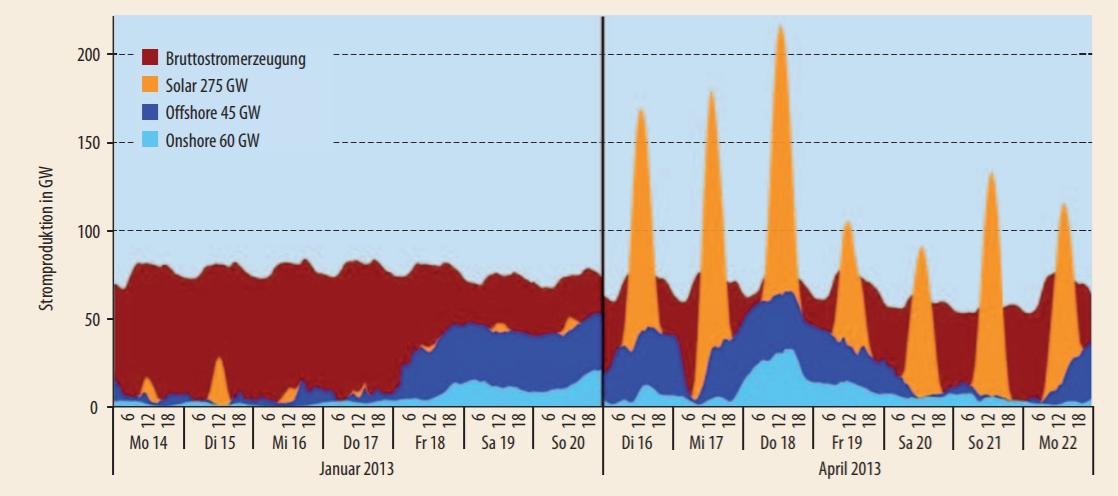
\includegraphics[width=1\textwidth]{images/DPG_Bild.PNG}
   \caption{Szenario bei ausgebauter EE-Stromproduktion im Jahr 2050 mit Wetterdaten aus dem Jahr 2013. \textbf{\textcolor{tugreen}{[9]}}}
\end{figure}
 \end{frame}



\begin{frame}{Paradigmenwechsel}
\begin{itemize}
  \item Stromindustrie und auch Verbraucher
  stehen vor bzw. befinden sich
  in einem Paradigmenwechsel hervorgerufen durch die Energiewende
\end{itemize}
%
 \begin{tabular}{p{0.5\textwidth}p{0.5\textwidth}}
 \textbf{\textcolor{tugreen}{ Ursprüngliche Situation:}}

 \begin{itemize}
     \item[-] Kraftwerkleistungen werden an Lastprofil angepasst
     \item[-] Lastprofil der Verbraucher bekannt und wenig fluktuierend
         \item[$\rightarrow$] geringe Schwankungen der Netz-Frequenz
         \item[$\rightarrow$] geringer Einsatz von Regelenergie
   \end{itemize}
 &
 \textbf{\textcolor{tugreen}{Neue Situation:}}
    \begin{itemize}
      \item[-] Erneuerbare Energie wird zum größten Teil aus volatilen Quellen wie Wind und Sonne gewonnen
      \item[-] Nur wenige grundlastfähige EE-Quellen wie Wasserkraft und Biogas
      \item[$\rightarrow$] EE-Kraftwerkleistungen nur noch bedingt oder gar nicht steuerbar
      \item[$\rightarrow$] keine Anpassung an Lastprofil möglich
      \item[$\rightarrow$] Netz-Frequenz fluktuierd stärker
      \item[$\rightarrow$] hoher Einsatz von Regelenergie, um Netzstabilität zu gewährleisten
    \end{itemize}\\
  \end{tabular}
\end{frame}


\begin{frame}{Folgen der Energiewende auf Stromnetz}
  \begin{tabular}{p{0.5\textwidth}p{0.5\textwidth}}
\textbf{\textcolor{tugreen}{Ursprüngliches Stromnetz:}}
\begin{itemize}
  \item Großkraftwerke wie z. B. Kern- oder Braunkohlekraftwerke,
  welche eine Region mit Strom versorgen
  \item "Einbahnstraße im Stromnetz"
\item[$\rightarrow$]  Kraftwerk$\rightarrow$Stromnetz$\rightarrow$Verbraucher
\item[$\rightarrow$]  Höchspannung$\rightarrow$Niederspannung
\end{itemize}
&
\textbf{\textcolor{tugreen}{Neues Stromnetz:}}

\begin{itemize}
  \item Erneuerbare Energiequellen können
  sowohl zentral z.B. Offshore Windparks als auch
  dezentral beim Verbraucher selbst
  produziert werden
\item[$\rightarrow$]  Kraftwerk$\rightarrow$Stromnetz$\leftrightarrows$Verbraucher
\item[$\rightarrow$]  Höchstspannung$\leftrightarrows$Niederspannung
\end{itemize}
\end{tabular}
\begin{itemize}
  % \textbf{\textcolor{tugreen}{Fazit:}}
\item[Fazit:] Notwendigkeit des Netz-um/aus-baus durch Energiewende,
damit eine sichere Versorgung gegeben bleibt
\item[$\rightarrow$] Netzentwicklungsplan NEP 2017-2030 der Bundesnetzagentur
\end{itemize}

\end{frame}



{
\setbeamertemplate{footline}{}
 \begin{frame}{Netzausbau}
%     \begin{figure}
%     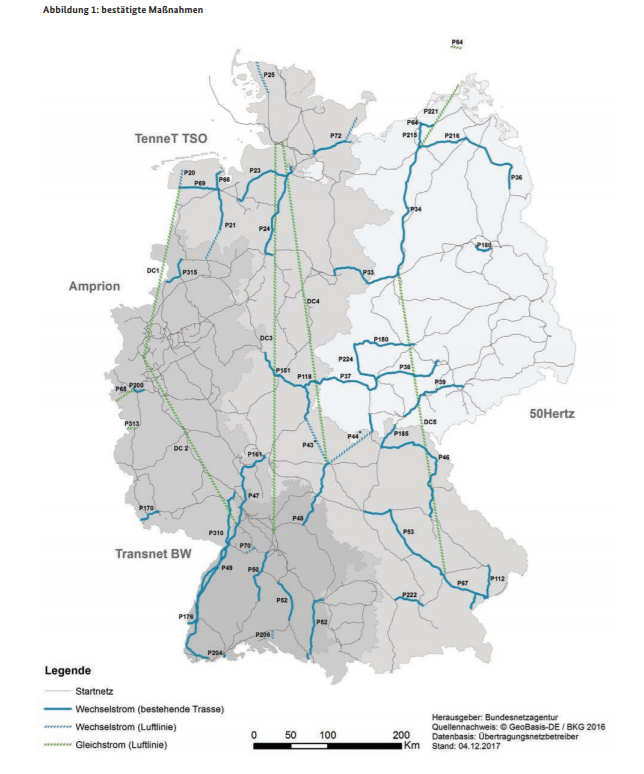
\includegraphics[width=0.55\textwidth]{images/Ausbau.PNG}
%   \end{figure}
\begin{overpic}[width=0.45\textwidth,tics=10]
{images/Ausbau.jpg}
\put(80,10){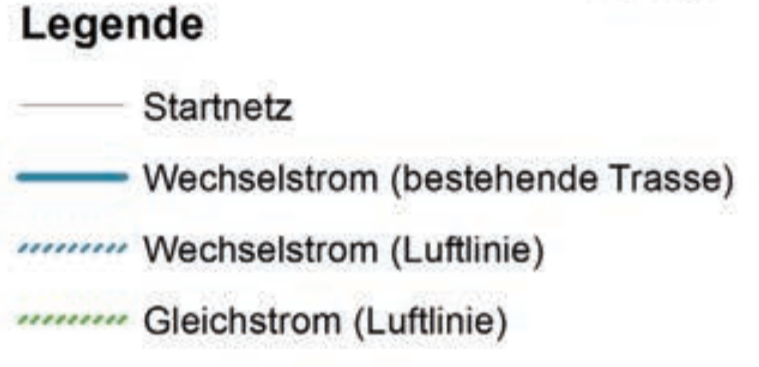
\includegraphics[scale=0.5]{images/Legende_deutschland.PNG}}
\put(75,5){\textbf{\textcolor{tugreen}{[10]}}}
\end{overpic}
\end{frame}
}





{
\setbeamertemplate{footline}{}
 \begin{frame}{Netzausbau}
%     \begin{figure}
%     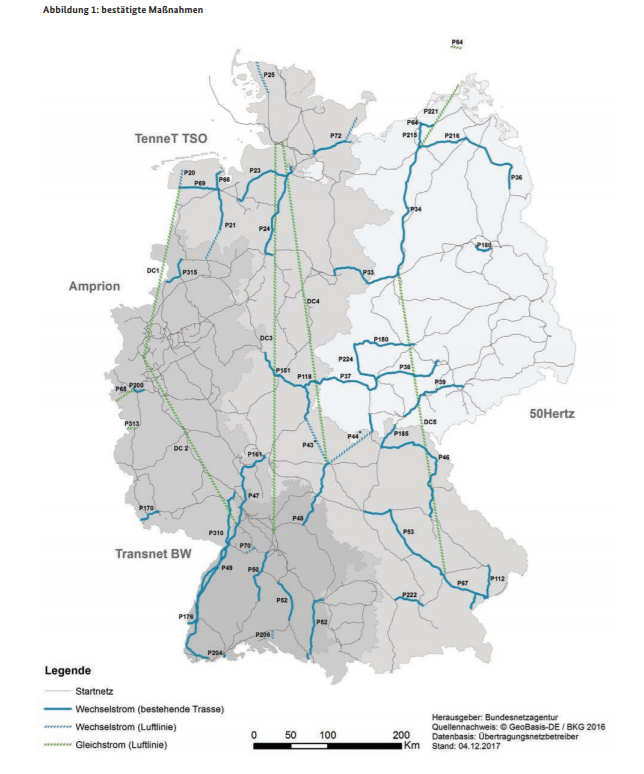
\includegraphics[width=0.55\textwidth]{images/Ausbau.PNG}
%   \end{figure}
\begin{overpic}[width=0.5\textwidth,tics=10]
{images/NAusbau1.jpg}
\put(80,10){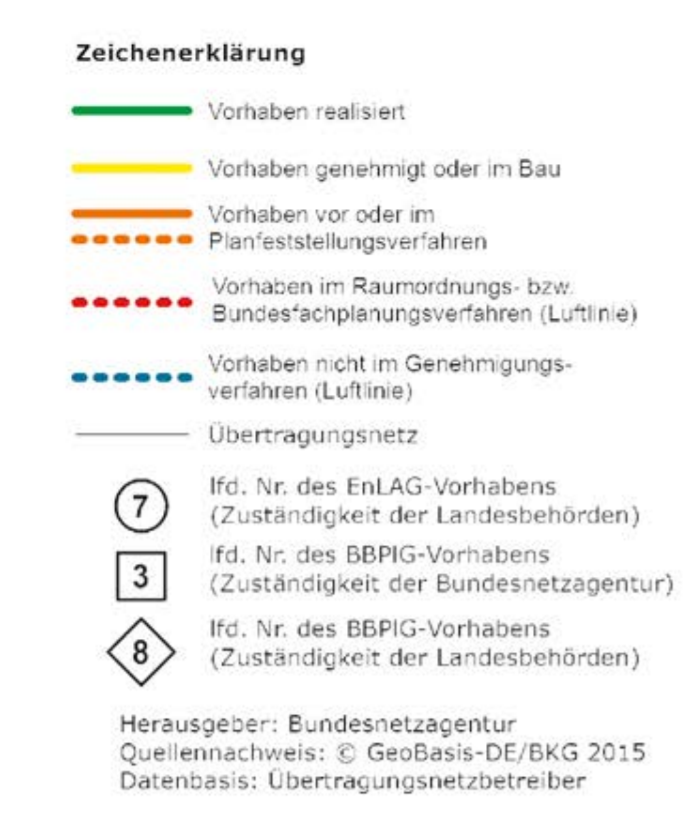
\includegraphics[scale=0.5]{images/NLegende.PNG}}
\put(80,5){\textbf{\textcolor{tugreen}{[11]}}}
\end{overpic}
\end{frame}
}

\begin{frame}{Zukunft Smart-Gird}
\begin{itemize}
  \item intelligentes Stromnetz durch Energiewende und
   die damit einhergehenden volatilen Stromerzeuger nötig
  \item Smart-Gird bietet Möglichkeit, den zu
  verfügungstehenden Strom effektiv zu nutzen
  \item Datenaustausch zwischen Netzbetreiber,
       Verbraucher und Erzeuger z. B. Smart-Meters in Haushalten
  \item[\rightarrow] mehr Kontrolle und Information
   für die Netzbetreiber für besseres Lastmanagement
   \item zusätzlich Anpassung der Nachfrage in Haushalten (Smart-Houses)
 \end{itemize}
\end{frame}

\begin{frame}
\begin{overpic}[width=1\textwidth]
  {images/smart-grid.jpg}
  \put(95,0){\textbf{\textcolor{tugreen}{[12]}}}
  %https://www.business.att.com/solutions/Service/internet-of-things/smart-cities/iot-smart-grid/
\end{overpic}
\end{frame}

\begin{frame}{Blackout}
  \begin{columns}
\begin{column}{0.5\textwidth}
\begin{itemize}
\item totaler Stromausfall mit regionalen bis überregionalen Auswirkungen
\item Ursachen:
\item[-]meist Vernachlässigung des N-1-Kriterium z.B. Ems-Freileitungskreuzung
\item[-]extreme Wetterbedingungen z.B. Münsterländer Schneechaos
\item[-]sabotierende Angriffe gegen Stromnetz oder Kraftwerke
   z.B. fiktiver Thriller "Blackout - Morgen ist es zu spät" von Marc Elsberg
\end{itemize}
\end{column}
\begin{column}{0.5\textwidth}
  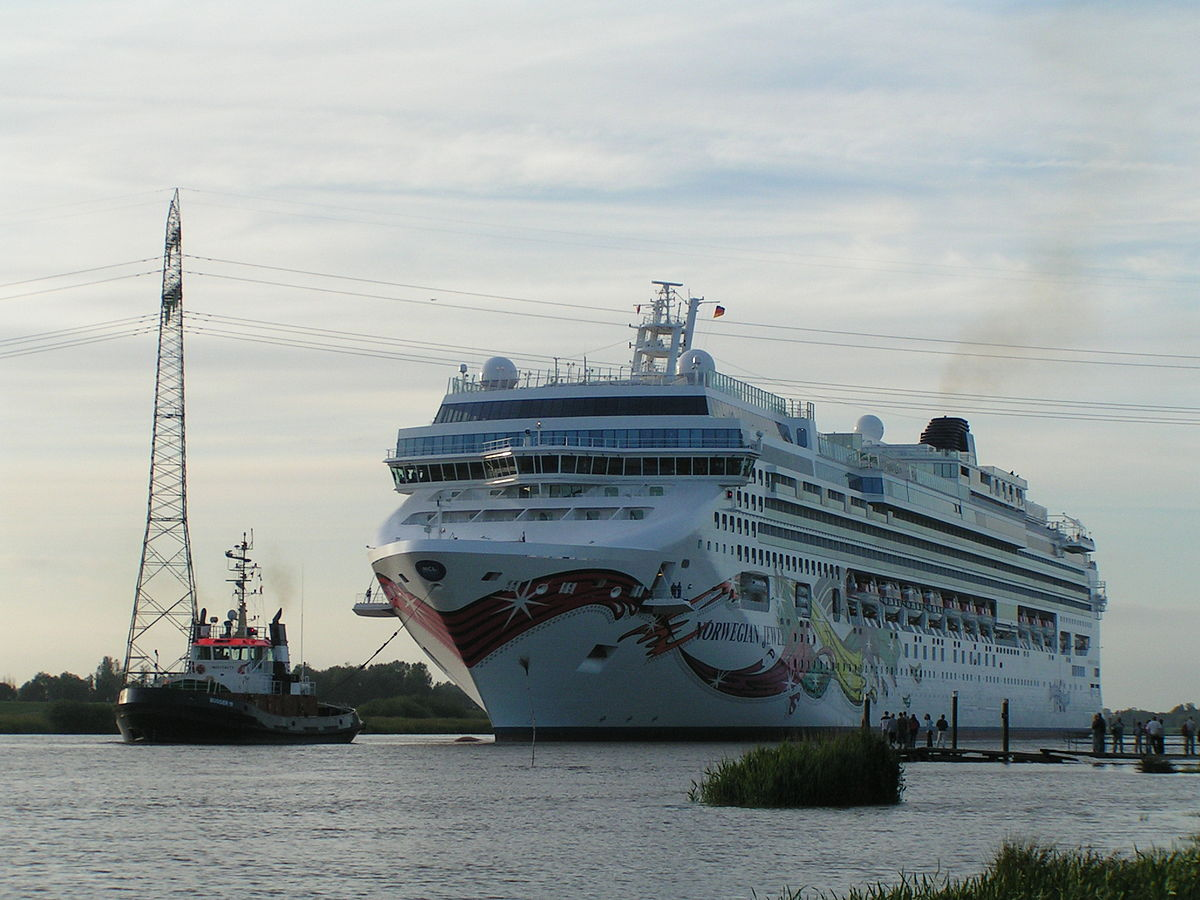
\includegraphics[width=0.8\textwidth]{images/Emsland_Bild.JPG} \ \textbf{\textcolor{tugreen}{[13]}}\\
  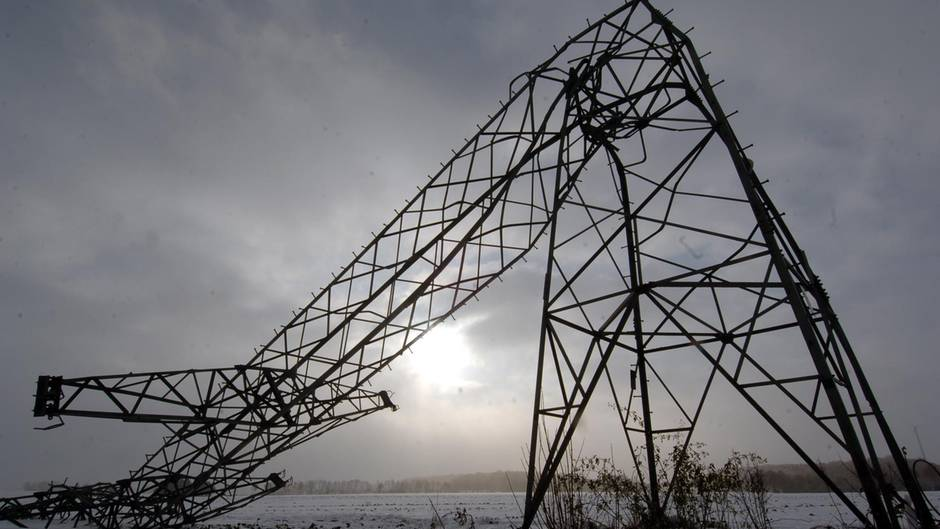
\includegraphics[width=0.8\textwidth]{images/stromausfall-deutschland-muensterland.jpg} \ \textbf{\textcolor{tugreen}{[14]}}\\
\end{column}
\end{columns}
\end{frame}





\begin{frame}{Strombörse}
\begin{itemize}
  \item existiert seit \num{2000} in Europa
  \item Strombörsen in Europa koordiniert von der EEX Group
  \item Deutschland, Frankreich, Österreich
  und Schweiz handeln an European Energy Exchange (EEX) in Leipzig
 und European Power Exchange (EPEX SPOT) in Paris
 \item Unterscheidung zwischen Spotmarkt, Terminmarkt und Regelenergiemarkt
\item Gehandelte Produkte zusätzlich zu Strom:
    \begin{itemize}
      \item[-]Öl, Gas, Kohle, Metall, Frachtprodukte,
       Emissionsberechtigungen sowie Agrarprodukte
    \end{itemize}
\end{itemize}
\end{frame}


{
\setbeamertemplate{footline}{}
\begin{frame}
  \centering
\begin{overpic}[width=1.1\textwidth]
  {images/stromprodukte.jpg}
\put(90,5){\textbf{\textcolor{tugreen}{[15]}}}
\end{overpic}
%Quelle:https://www.next-kraftwerke.de/wissen/strommarkt/spotmarkt-epex-spot
\end{frame}
}

\begin{frame}{Spotmarkt}
  \begin{columns}
  \begin{column}{0.3\textwidth}
  \begin{itemize}
    \item Spotmarkt in Paris an der EPEX SPOT
    \item Handel von kurzfristig lieferbaren Strommengen in bestimmten Blöcken
    \item Im Intraday-Handel (Lieferung am selben Tag)
    \item Im Day-Ahead-Handel (Lieferung am Folgetag)
  \end{itemize}
  \end{column}
  \begin{column}{0.7\textwidth}
\centering
  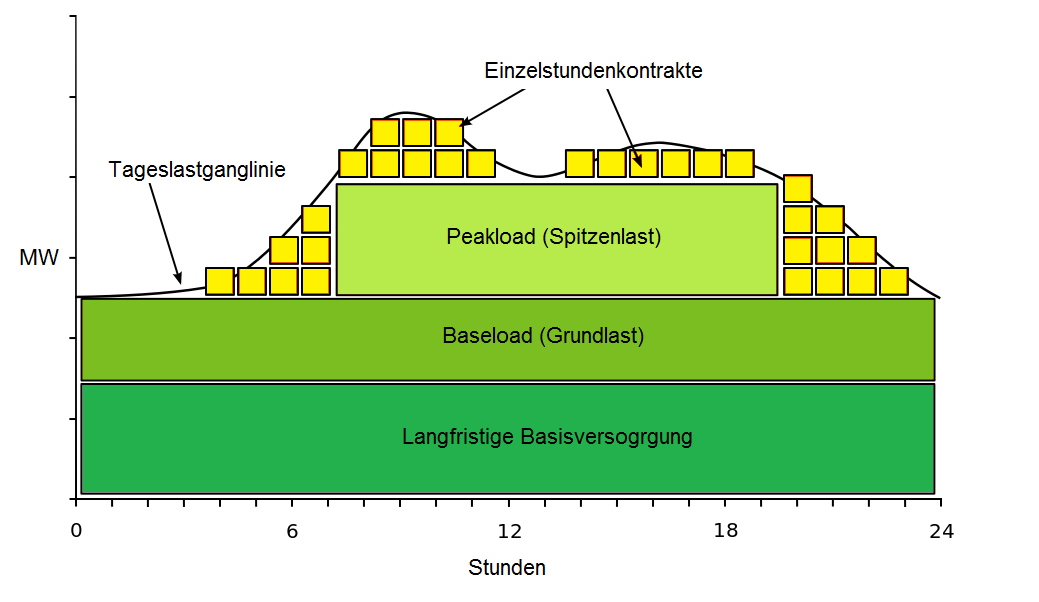
\includegraphics[width=1\textwidth]{images/Stromborse_stromverbrauch_lastprofil.png} \ \textbf{\textcolor{tugreen}{[16]}}
\end{column}
\end{columns}
\end{frame}


\begin{frame}{Merit-Order}
\begin{itemize}
  \item Beschreibungsmodell der Preisbildung auf dem Strommarkt
  \item orientiert sich an den Grenzkosten der Kraftwerke
  (Grenzkosten entspricht Kosten für die letzte produzierte Megawattstunde)
\item Kraftwerke mit niedrigen Grenzkosten werden bei der
 Einspeisung bevorzugt, bis Nachfrage gedeckt ist
\item Börsenpreis ergibt sich aus Schnittstelle von Angebot und Nachfrage
\begin{itemize}
  \item[$\rightarrow$] Grenzkosten des Kraftwerkes, welches zuletzt den
  Zuschlag zur Einspeisung erhält, definiert Börsenpreis für alle eingespeisten Kraftwerke("uniform pricing")
\end{itemize}
\end{itemize}
\centering
\begin{overpic}[width=0.5\textwidth]
  {images/Merit_Order_2008.PNG}
  \put(90,5){\textbf{\textcolor{tugreen}{[17]}}}
\end{overpic}
\end{frame}

\begin{frame}
  \begin{overpic}[width=1\textwidth]
    {images/Meritorder.png}
    \put(100,2){\textbf{\textcolor{tugreen}{[18]}}}
\end{overpic}
%Quelle:https://www.next-kraftwerke.be
\end{frame}

\begin{frame}
  \begin{overpic}[width=1\textwidth]
    {images/Merit.png}
    \put(95,2){\textbf{\textcolor{tugreen}{[19]}}}
\end{overpic}
%Quelle:https://www.next-kraftwerke.be
\end{frame}


\begin{frame}{Spotmarktpreis 20.1.2018}
  \begin{overpic}[width=0.9\textwidth]
    {images/10_1_2018_spot.PNG}
\put(94,4){\textbf{\textcolor{tugreen}{[20]}}}
\end{overpic}
\end{frame}

\begin{frame}{Terminmarkt}
\begin{itemize}
  \item Terminmarkt in Leipzig an der EEX
  \item Handel von Strommengen, die zu einem festen Termin zu Verfügung gestellt werden (Strom-Futures)
  \item bis zu 6 Jahre Strom im voraus kaufen
  \item Jahr-, Quartal-, Monat-, Woche-,  Wochenende- und Tag-Kontrakte
  \item Preis richtet sich nach Börsenindex der Strombörse z. B. Phelix (Physical Electricity Index)
\end{itemize}
\end{frame}

\begin{frame}{Phelix}
  \begin{overpic}[width=0.9\textwidth]
    {images/Phelix_1monat.PNG}
\put(94,4){\textbf{\textcolor{tugreen}{[21]}}}
\end{overpic}
\end{frame}


\begin{frame}{Regelenergiemarkt}
\begin{itemize}
  \item Bedarf an Regelenergien von PRL, SRL und MRL werden durch Ausschreibung
der ÜNB gedeckt
\item PRL und SRL werden jede Woche neu ausgeschrieben
\item MRL werden täglich neu ausgeschrieben und nach Merit-Order-Liste bei Bedarf abgerufen
\item Preis abhängig von Verträgen zwischen Anbieter und ÜNB
\end{itemize}
\end{frame}

{
\setbeamertemplate{footline}{}
\begin{frame}
  \centering
  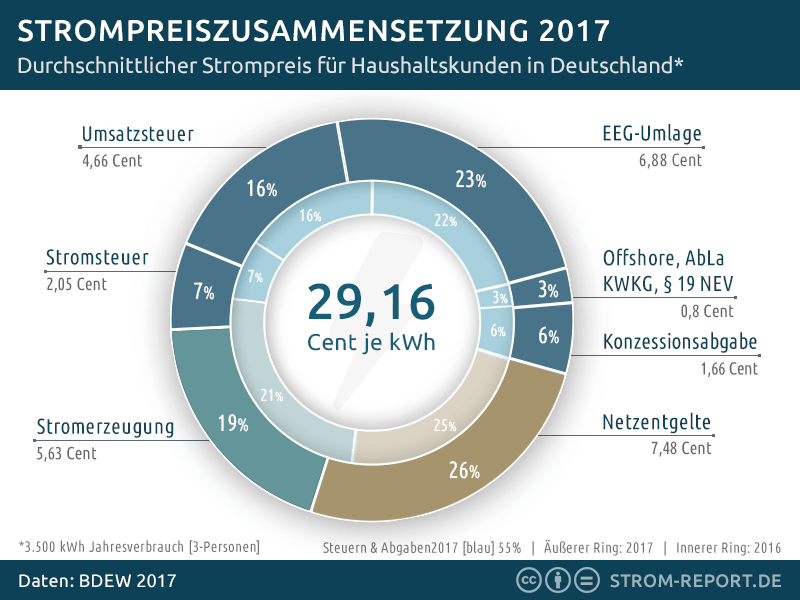
\includegraphics[width=0.8\textwidth]{images/strompreis-zusammensetzung.png} \ \textbf{\textcolor{tugreen}{[22]}}
\end{frame}
}


\begin{frame}{Erneuerbare-Energien-Gesetz EEG}
   \begin{itemize}
     \item das EEG wurde im Jahr 2000 eingeführt und mehrmals überarbeitet aktuell EEG 2017
   \end{itemize}
    \begin{block}{Ziel:}
      Förderung von Erneuerbaren Energiequellen, damit Umstieg von Konventionellen zur Erneuerbaren Energiequellen gelingt
    \end{block}
  %\item Regelt die Einspeisung des EE-Stromes
    \begin{block}{Maßnahmen des EEG zu Förderung von EE-Strom:}
     \begin{itemize}
       \item[$\rightarrow$] Verpflichtung an die Netzbetreiber EE-Anlagen an das Stromnetz anzuschießen und EE-Strom vorrangig einzuspeisen
       \item[$\rightarrow$] garantierte Einspeisevergütung des EE-Stromes an die Anlagenbetreiber durch den Netzbetreiber für 20 Jahre
   \end{itemize}
   \end{block}
\end{frame}

\begin{frame}{Auswirkungen des EEG}
  \begin{itemize}
    \item Abnahmepflicht fördert Merit-Order-Effekt
    \item Netzbetreiber bieten abgenommenen EE-Strom an der Börse an
\begin{itemize}
  \item[$\rightarrow$] Gewinn an der Strombörse deckt jedoch nicht die vollen Vergütungskosten der Netzbetreiber
\end{itemize}
\end{itemize}
\begin{block}{EEG-Umlage}
\begin{itemize}
  \item $\text{EEG-Umlage}=\text{Einspeisevergütung}-\text{Börsengewinn}$
\item die EEG-Umlage erhält der Netzbetreiber von allen Stromverbrauchern
\item Strompreis enthält die EEG-Umlage
\end{itemize}
\end{block}
\end{frame}

{
\setbeamertemplate{footline}{}
\begin{frame}
\centering
  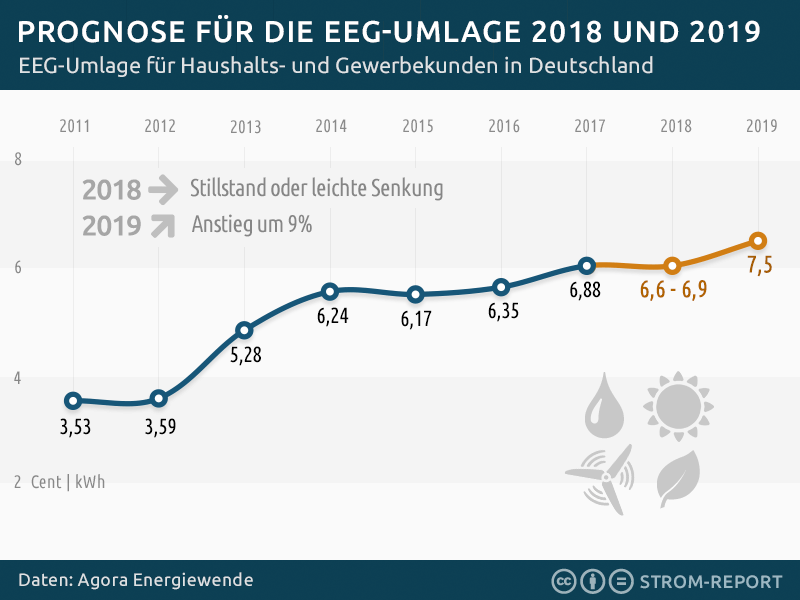
\includegraphics[width=0.8\textwidth]{images/eeg-umlage-2018-2019.png} \ \textbf{\textcolor{tugreen}{[23]}}
%Quelle:https://1-stromvergleich.com/strom-report/eeg-umlage/#eeg-umlage-2018
\end{frame}
}




{
\setbeamertemplate{footline}{}
\begin{frame}
  \centering
  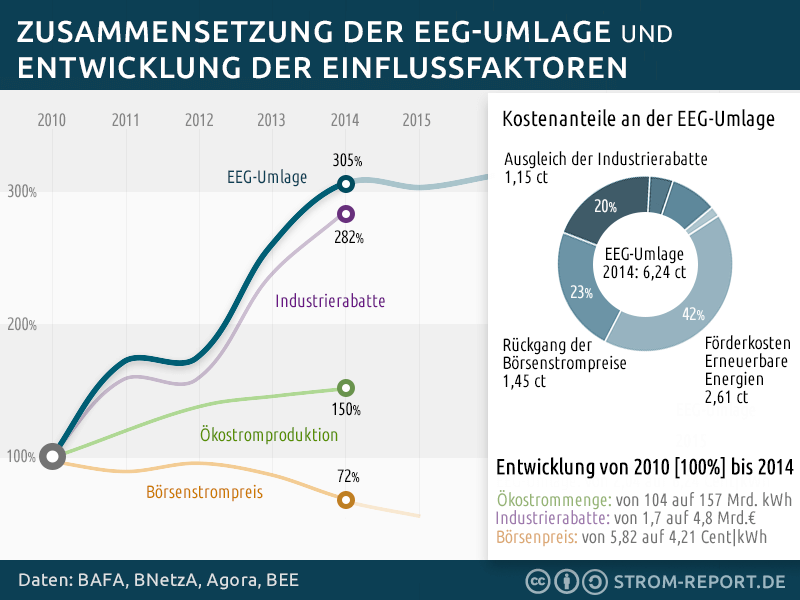
\includegraphics[width=0.8\textwidth]{images/eeg-umlage.png} \ \textbf{\textcolor{tugreen}{[24]}}
%Quelle:https://1-stromvergleich.com/strom-report/eeg-umlage/#eeg-umlage-boersenpreis-industrierabatt
\end{frame}
}




\begin{frame}{Zusammenfassung}
\begin{tabular}{p{0.4\textwidth}p{0.6\textwidth}}
   Stormnetz  &         Strombörse\\
\begin{itemize}
  \item Dreiphasiger Wechselstrom in Verbundnetzen
  \item 4 Spannungsebenen
  \item keine Energiespeicherung im Netz selber möglich
  \item Netzfrequenz durch Regelleistung geregelt
  \item Paradigmenwechsel in der Stromindustrie durch Energiewende
  \item Netzausbau und neue Konzepte nötig um Energiewende zu bewergstellen
\end{itemize}

&
\begin{itemize}
  \item Unterscheidung zwischen Spot-, Termin- und Regelenergiemarkt
  \item Preisbildung an dem Spotmarkt durch die Merit-Order
  \item Merit-Order-Effekt durch EE
  \item EEG als Beschleuniger der Energiewende und dessen Folgen
\end{itemize}

\end{tabular}
\end{frame}





\begin{frame}{Quellen}
\begin{itemize}
  \item \url{https://www.next-kraftwerke.de/wissen}
  \item \url{https://de.wikipedia.org/wiki/Netzfrequenz}
  \item \url{https://www.netzfrequenz.info/}
\item \url{https://de.wikipedia.org/wiki/Stromnetz}
\item \url{https://www.weltderphysik.de/gebiete/technik/energie/speichern-und-transportieren/strom/hochspannung/}
\item \url{http://www.energie.ch/drehstrom-und-wechselstrom}
\item \url{https://www.umweltbundesamt.de/service/uba-fragen/was-ist-ein-smart-grid}
\item \url{https://de.wikipedia.org/wiki/Hochspannungs-Gleichstrom-Übertragung}
\item \url{https://www.eex.com/blob/63996/60aa085313f902cbbb8ca9cbb6db622b/neu-d-eex-broschuere-2017-web-data.pdf}
\item \url{https://de.wikipedia.org/wiki/Merit-Order}
\item \url{https://de.wikipedia.org/wiki/Strombörse}
\item \url{https://de.wikipedia.org/wiki/Europäisches_Verbundsystem}
\item \url{http://www.bpb.de/politik/wirtschaft/energiepolitik/148524/ausbau-des-stromnetzes}
% \item \url{}
\end{itemize}
\end{frame}

\begin{frame}{Bildquellen}
  \begin{tabular}{p{0.02\textwidth}p{0.98\textwidth}}
&
 \begin{itemize}
   \item[{[1]}]  \url{http://www.c-turbines.ch/generator.html}
   \item[{[2]}] \url{https://commons.wikimedia.org/w/index.php?curid=1387849}
   \item[{[3]}] \url{https://de.wikipedia.org/wiki/Hochspannungs-Gleichstrom-Übertragung}
   \item[{[4],[10]}] \url{https://www.netzausbau.de/SharedDocs/Downloads/DE/Publikationen/ZFBedarfsermittlung2030.pdf?__blob=publicationFile}
\item[{[5]}]  \url{https://de.wikipedia.org/wiki/Stromnetz}
\item[{[6]}]  \url{http://www.bpb.de/politik/wirtschaft/energiepolitik/148524/ausbau-des-stromnetzes}
\item[{[7]}]  \url{http://www.netzfrequenz.info/aktuelle-netzfrequenz-full}
\item[{[8]}]  \url{https://fenecon.de/page/stromspeicher-energy-pool}
\item[{[9]}]  entnommen aus Physik Journal Nr. 12 (2013), Viley-VCH Verlag
\item[{[11]}] \url{http://www.bmwi.de/Redaktion/DE/Publikationen/Energie/strom-2030-ergebnispapier.pdf?__blob=publicationFile&v=32}
\item[{[12]}] \url{https://www.business.att.com/solutions/Service/internet-of-things/smart-cities/iot-smart-grid/}
\end{itemize}
\\
\end{tabular}
\end{frame}

\begin{frame}{Bildquellen}
  \begin{tabular}{p{0.02\textwidth}p{0.98\textwidth}}
&
 \begin{itemize}
\item[{[13]}] \url{https://commons.wikimedia.org/wiki/File:Mittling-Mark_Norwegian_Jewel.JPG}
\item[{[14]}] \url{https://image.stern.de/7788040/16x9-940-529/322870288dd4910ab3be3785e2dd5533/aw/stromausfall-deutschland-muensterland.jpg}
\item[{[15]}] \url{https://www.next-kraftwerke.de/wissen/strommarkt/spotmarkt-epex-spot}
\item[{[16]}] Grundlage: \url{http://deacademic.com/dic.nsf/dewiki/830500}
\item[{[17]}]  \url{https://de.wikipedia.org/wiki/Merit-Order}
\item[{[18],[19]}] \url{https://www.next-kraftwerke.de/wissen/strommarkt/merit-order}
\item[{[20],[21]}] \url{https://www.epexspot.com/de/marktdaten}
\item[{[22]}] \url{https://1-stromvergleich.com/download/zusammensetzung-strompreis-2017/}
\item[{[23],[24]}] \url{https://1-stromvergleich.com/strom-report/eeg-umlage/}
\end{itemize}
\\
\end{tabular}

\end{frame}


\begin{frame}{Backup}

\end{frame}


{
\setbeamertemplate{footline}{}
\begin{frame}
  \begin{figure}
    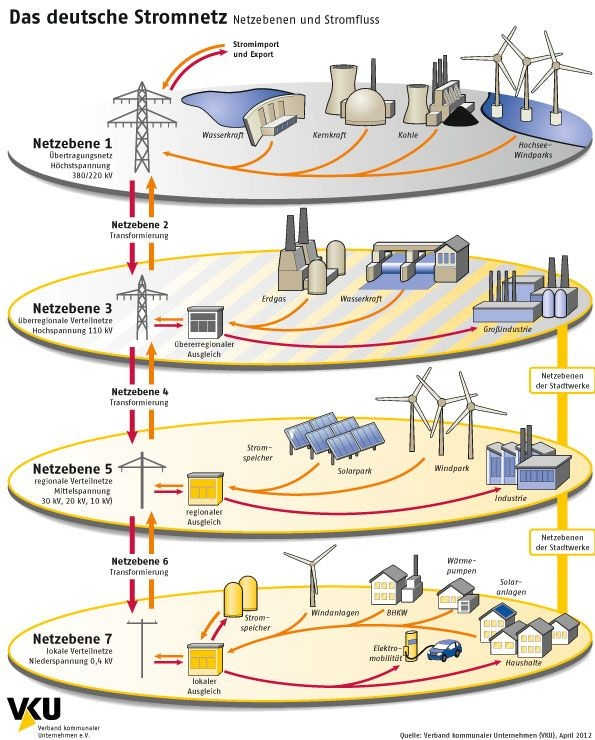
\includegraphics[width=0.4\textwidth]{images/netzebenen.jpg}
    %Quelle: http://www.bpb.de/politik/wirtschaft/energiepolitik/148524/ausbau-des-stromnetzes
  \end{figure}
\end{frame}
}

%
% {
% \setbeamertemplate{footline}{}
% \begin{frame}
%   \begin{figure}
%   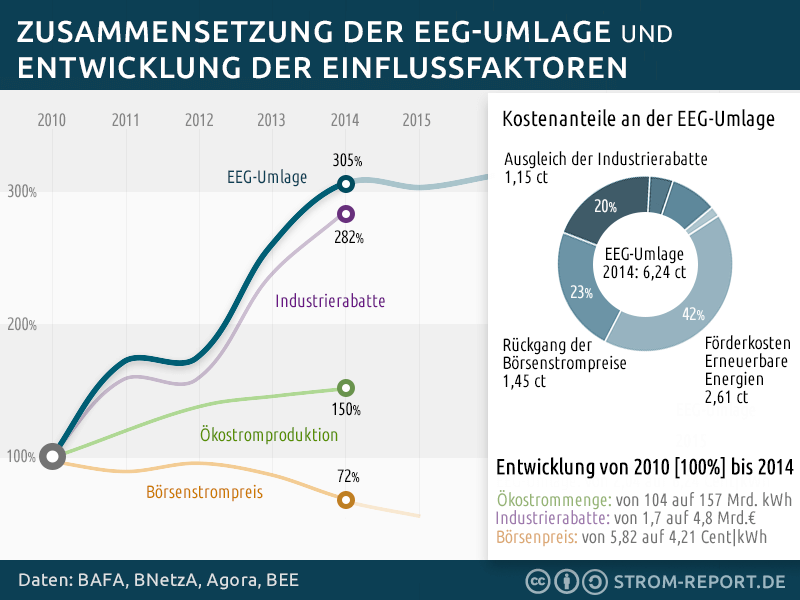
\includegraphics[width=0.9\textwidth]{images/eeg-umlage.png}
%   \end{figure}
% %Quelle:https://1-stromvergleich.com/strom-report/eeg-umlage/#eeg-umlage-boersenpreis-industrierabatt
% \end{frame}
% }




\end{document}
